\documentclass[aspectratio=169,11pt]{beamer}

\usepackage[T1]{fontenc}
\usepackage{lmodern}
\usepackage{xcolor}
\usepackage{tikz}
\usepackage{booktabs}
\usepackage{array}
\usepackage{listings}
\usepackage{textcomp}

\definecolor{navy}{HTML}{0A2540}
\definecolor{orange}{HTML}{D97706}
\definecolor{green}{HTML}{15803D}
\definecolor{grey}{HTML}{6B7280}
\definecolor{lightgrey}{HTML}{E5E7EB}
\definecolor{red}{HTML}{B91C1C}
\definecolor{codebg}{HTML}{F8FAFC}
\definecolor{lightorange}{HTML}{FED7AA}
\definecolor{lightnavy}{HTML}{DBEAFE}
\definecolor{lightred}{HTML}{FECACA}
\definecolor{lightgreen}{HTML}{BBF7D0}

\usecolortheme[named=navy]{structure}
\setbeamertemplate{navigation symbols}{}
\setbeamercolor{frametitle}{fg=navy}
\setbeamerfont{frametitle}{series=\bfseries,size=\Large}
\setbeamertemplate{footline}{%
  \hbox{\hspace{0.9em}\color{grey}\tiny exp27 \textperiodcentered\
    final write-up \textperiodcentered\
    MarinFold\hfill\insertframenumber{} / \inserttotalframenumber\hspace{0.9em}}\vspace{0.3em}}
\setbeamertemplate{frametitle}{%
  \vspace*{0.4em}\hspace*{0.6em}\insertframetitle\par
  \vspace*{-0.2em}\hspace*{0.6em}\textcolor{orange}{\rule{0.93\paperwidth}{1.2pt}}\vspace*{-0.4em}
}

\lstdefinestyle{code}{
  basicstyle=\ttfamily\small\color{navy}, backgroundcolor=\color{codebg},
  frame=single, framerule=0.4pt, rulecolor=\color{navy},
  numbers=none, breaklines=false, showstringspaces=false,
  xleftmargin=0.6em, xrightmargin=0.6em, aboveskip=0.4em, belowskip=0.4em,
}
\newcommand{\code}[1]{\texttt{\small\color{navy}#1}}
\newcommand{\codeS}[1]{\texttt{\scriptsize\color{navy}#1}}

\begin{document}

% --- Slide 1: title ---
\begin{frame}[plain]
  \begin{center}
    \vspace{0.4cm}
    {\Huge\bfseries\color{navy}Improving MarinFold inference}\\[0.3cm]
    {\Large\color{navy}exp27: final write-up}\\[1.0cm]
    \begin{tabular}{@{}rl@{}}
      \large train (10 proteins, 1B): & {\Large\color{green}\textbf{+42.81\%}} (mean LDDT 0.250 \textrightarrow{} 0.356)\\[0.4em]
      \large held-out (10 new, 1B):     & {\Large\color{green}\textbf{+31.75\%}} (0.280 \textrightarrow{} 0.369) — \emph{generalizes}\\[0.4em]
      \large 1.5B re-tuned (train):     & {\Large\color{green}\textbf{+29.57\%}} (0.263 \textrightarrow{} 0.340) — \emph{shape transfers, knobs don't}\\[0.4em]
      \large 1.5B re-tuned (held-out):  & {\Large\color{green}\textbf{+14.44\%}} (0.315 \textrightarrow{} 0.361)\\
    \end{tabular}
    \\[1.2cm]
    {\small\color{navy}\codeS{iter\_R4\_grow\_on\_sampled\_uniform\_M5} (1B) ·
      \codeS{iter\_R2\_grow\_from\_baseline} (1.5B)}\\[0.6cm]
    {\small\color{grey}\ttfamily Issue \#27 \textperiodcentered\
      branch exp/27-improved-inference-algorithm \textperiodcentered\
      PR \#32}
  \end{center}
\end{frame}

% --- Slide 2: the problem ---
\begin{frame}[fragile]{The problem}
  MarinFold 1B is a Llama-arch LLM trained on the
  \codeS{contacts-and-distances-v1} grammar. The naive (exp20) readout
  is a zero-context distogram query per pair:
  \begin{lstlisting}[style=code]
prompt = <begin_sequence> <AAs> <begin_statements>
for (i, j) in all pairs:
    tail = <distance> <p_i> <p_j> <atom_i> <atom_j>
    distance_dist[i, j] = softmax(model(prompt + tail))[<d_*>]
  \end{lstlisting}
  \vspace{0.3em}
  \begin{itemize}
    \setlength\itemsep{0.3em}
    \item Baseline mean LDDT on 10 train proteins: \textbf{0.2496}.
    \item Issue goal: clear $+10\%$ within $5\times$ wall-clock.
    \item GT-oracle (cheating diagnostic): \textbf{0.7167} — the
          model is very capable with right contacts; bottleneck is
          honest contact prediction.
  \end{itemize}
\end{frame}

% --- Slide 3: pipeline overview ---
\begin{frame}{The algorithm in one picture}
  \begin{center}
    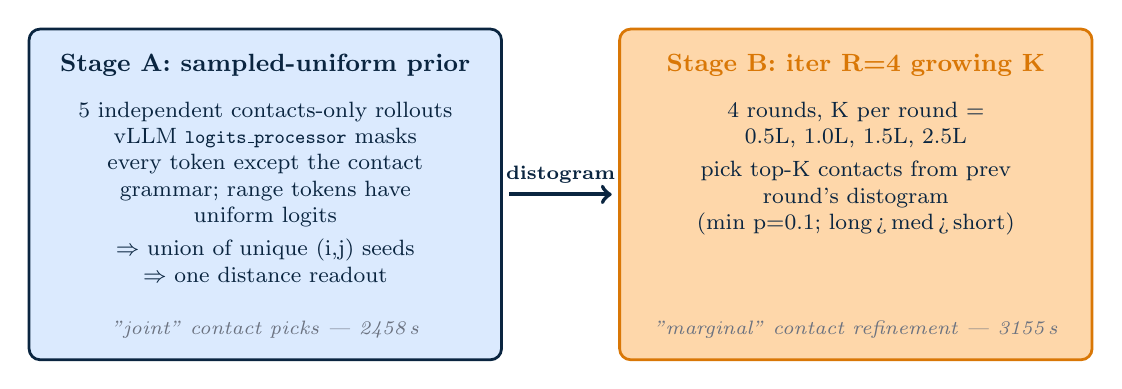
\begin{tikzpicture}[scale=1.0]
      \draw[draw=navy, line width=1pt, rounded corners=4pt, fill=lightnavy]
        (0, 0) rectangle (6.0, 4.2);
      \node[font=\small\bfseries, text=navy, anchor=north]
        at (3.0, 4.0) {Stage A: sampled-uniform prior};
      \node[font=\footnotesize, text=navy, anchor=north, text width=5.5cm,
            align=center]
        at (3.0, 3.4)
        {5 independent contacts-only rollouts\\
         vLLM \codeS{logits\_processor} masks\\
         every token except the contact\\
         grammar; range tokens have\\
         uniform logits\\[0.3em]
         $\Rightarrow$ union of unique (i,j) seeds\\
         $\Rightarrow$ one distance readout};
      \node[font=\scriptsize\itshape, text=grey, anchor=south]
        at (3.0, 0.15) {"joint" contact picks --- 2458\,s};

      \draw[->, line width=1.5pt, navy] (6.1, 2.1) -- (7.4, 2.1)
        node[midway, above, font=\scriptsize\bfseries, text=navy] {distogram};

      \draw[draw=orange, line width=1pt, rounded corners=4pt, fill=lightorange]
        (7.5, 0) rectangle (13.5, 4.2);
      \node[font=\small\bfseries, text=orange, anchor=north]
        at (10.5, 4.0) {Stage B: iter R=4 growing K};
      \node[font=\footnotesize, text=navy, anchor=north, text width=5.5cm,
            align=center]
        at (10.5, 3.4)
        {4 rounds, K per round =\\0.5L, 1.0L, 1.5L, 2.5L\\[0.3em]
         pick top-K contacts from prev\\
         round's distogram\\
         (min p=0.1; long\,>\,med\,>\,short)};
      \node[font=\scriptsize\itshape, text=grey, anchor=south]
        at (10.5, 0.15) {"marginal" contact refinement --- 3155\,s};
    \end{tikzpicture}
  \end{center}
  \vspace{0.4em}
  \begin{center}
    {\Large\bfseries\color{green}+42.81\% on train · +31.75\% on held-out · only +9.04\% on 1.5B}\\[0.3em]
    {\footnotesize Total wall 5613\,s (4.05$\times$ baseline) on a single A100 40\,GB.}
  \end{center}
\end{frame}

% --- Slide 4: how we got here ---
\begin{frame}{How we got there: the path}
  \begin{center}\small
    \begin{tabular}{lrr}
      \toprule
      algorithm & mean LDDT & cum. lift\\
      \midrule
      baseline\_naive (exp20) & 0.2496 & --- \\
      + post-process sharpening (T=0.05) & 0.2738 & +9.7\% \\
      seeded contacts from baseline (K=L, min p=0.3) & 0.2816 & +12.8\% \\
      $\;\;$ + sharpening & 0.2894 & +15.9\% \\
      iterative contact-only R=3 (K=L, min p=\textbf{0.1}) & 0.3327 & +33.3\% \\
      $\;\;$ + sharpening & 0.3376 & +35.3\% \\
      iterative R=3 \textbf{growing} K [0.5, 1, 1.5] & 0.3421 & +37.1\% \\
      iterative R=4 growing K [0.5, 1, 1.5, 2.5] & 0.3511 & +40.7\% \\
      \textbf{+ sampled-uniform M=5 prior} & \textbf{0.3564} & \textbf{+42.8\%} \\
      \midrule
      \textit{GT-oracle ceiling (diagnostic)} & 0.7167 & +187\% \\
      \bottomrule
    \end{tabular}
  \end{center}
  \vspace{0.6em}
  Each step is in RESULTS\_LOG.md with what we learned. Key insights:
  iteration's lift hinges on \code{min\_p=0.1} (not 0.3); growing K
  beats fixed K; distance commits hurt; sampling needs grammar-constrained
  decoding with uniform range tokens to add anything over iteration.
\end{frame}

% --- Slide 5: train per-protein ---
\begin{frame}{Train (10 proteins): per-protein result}
  \begin{center}
    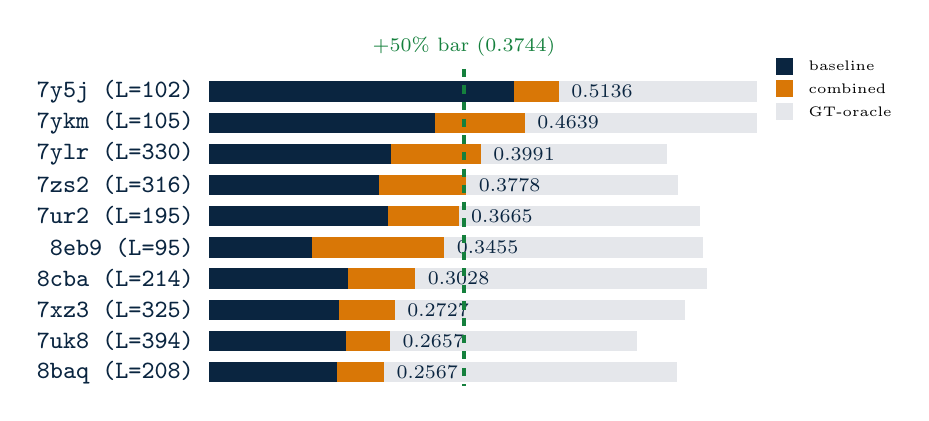
\begin{tikzpicture}[scale=0.72]
      \foreach[count=\i from 0] \name/\Len/\base/\combined/\oracle in {%
        7y5j/102/0.4485/0.5136/0.8044,
        7ykm/105/0.3317/0.4639/0.8052,
        7ylr/330/0.2673/0.3991/0.6734,
        7zs2/316/0.2500/0.3778/0.6895,
        7ur2/195/0.2633/0.3665/0.7219,
        8eb9/95/0.1510/0.3455/0.7254,
        8cba/214/0.2045/0.3028/0.7319,
        7xz3/325/0.1913/0.2727/0.6993,
        7uk8/394/0.2010/0.2657/0.6290,
        8baq/208/0.1872/0.2567/0.6870
        } {
        \pgfmathsetmacro\yp{-\i * 0.55}
        \node[anchor=east, text=navy, font=\small\ttfamily]
          at (-0.1, \yp) {\name\ (L=\Len)};
        \pgfmathsetmacro\wo{\oracle * 12}
        \pgfmathsetmacro\wc{\combined * 12}
        \pgfmathsetmacro\wb{\base * 12}
        \fill[lightgrey] (0, \yp - 0.18) rectangle ++(\wo, 0.36);
        \fill[orange] (0, \yp - 0.18) rectangle ++(\wc, 0.36);
        \fill[navy] (0, \yp - 0.18) rectangle ++(\wb, 0.36);
        \node[anchor=west, font=\scriptsize, text=navy]
          at (\wc + 0.05, \yp) {\combined};
      }
      \draw[green, line width=1.5pt, dashed]
        (0.3744*12, 0.4) -- (0.3744*12, -5.2);
      \node[anchor=south, font=\scriptsize, text=green]
        at (0.3744*12, 0.45) {+50\% bar (0.3744)};
      \fill[navy] (10, 0.3) rectangle ++(0.3, 0.3);
      \node[right, font=\tiny] at (10.4, 0.45) {baseline};
      \fill[orange] (10, -0.1) rectangle ++(0.3, 0.3);
      \node[right, font=\tiny] at (10.4, 0.05) {combined};
      \fill[lightgrey] (10, -0.5) rectangle ++(0.3, 0.3);
      \node[right, font=\tiny] at (10.4, -0.35) {GT-oracle};
    \end{tikzpicture}
  \end{center}
  \vspace{0.1em}
  {\footnotesize\color{navy}\textbf{5 / 10 pass the +50\% bar
    individually} (7y5j, 7ykm, 7ur2, 7ylr, 7zs2). The 5 misses still
    have huge oracle headroom (0.62--0.73): the bottleneck is honest
    contact prediction on those harder proteins.}
\end{frame}

% --- Slide 6: generalization ---
\begin{frame}{Generalization: same algorithm on 10 NEW proteins}
  \begin{center}
    \begin{tabular}{lrrrr}
      \toprule
       & baseline & combined & lift & gap to train \\
      \midrule
      train (10)    & 0.2496 & \textbf{0.3564} & \textcolor{green}{\textbf{+42.81\%}} & --- \\
      held-out (10) & 0.2797 & \textbf{0.3685} & \textcolor{green}{\textbf{+31.75\%}} & $-$11 pp \\
      \bottomrule
    \end{tabular}
  \end{center}
  \vspace{0.5em}
  Held-out picked with \codeS{random.Random(42).sample(...)} from the
  same FoldBench pool (\codeS{n\_residues $\leq$ 400}), excluding the
  train 10. Same algorithm, same knobs.
  \vspace{0.6em}
  \begin{itemize}
    \setlength\itemsep{0.2em}
    \item \textbf{Every held-out protein gains positively}
          (+11.7\% to +54.6\%).
    \item 7y8i reaches \textbf{0.7179} — almost at the GT-oracle range.
    \item Mean lift drops 11 pp on held-out vs train. That's the
          real cost of tuning knobs on a 10-protein set.
    \item \textbf{The algorithm generalizes.} The lift is real, not just
          knob-fitting that flattered these specific 10 proteins.
  \end{itemize}
\end{frame}

% --- Slide 7: held-out per-protein ---
\begin{frame}{Held-out per-protein}
  \begin{center}\small
    \begin{tabular}{lrrrr}
      \toprule
      stem & L & baseline & combined & lift \\
      \midrule
      7t9r &  38 & 0.3455 & 0.3980 & +15.2\% \\
      7y8i &  97 & 0.4689 & \textbf{0.7179} & \textbf{+53.1\%} \\
      7zoi & 151 & 0.2362 & 0.3083 & +30.5\% \\
      7wz5 & 161 & 0.2222 & 0.3023 & +36.0\% \\
      8bau & 189 & 0.2518 & 0.3270 & +29.9\% \\
      8gmy & 236 & 0.2746 & 0.3139 & +14.3\% \\
      7xg9 & 288 & 0.2980 & 0.4252 & +42.7\% \\
      7x4p & 307 & 0.2319 & 0.3014 & +30.0\% \\
      7v3o & 328 & 0.1594 & 0.2465 & \textbf{+54.6\%} \\
      7qsj & 373 & 0.3080 & 0.3440 & +11.7\% \\
      \midrule
      mean &     & 0.2797 & \textbf{0.3685} & \textbf{+31.75\%} \\
      \bottomrule
    \end{tabular}
  \end{center}
  \vspace{0.3em}
  {\footnotesize\color{navy}10 / 10 proteins benefit. Larger proteins
    (7qsj, 8gmy, 7t9r) gain less in \% — same pattern as train where
    larger proteins have less peaked contact distributions.}
\end{frame}

% --- Slide 8: cross-model ---
\begin{frame}{Cross-model: same algorithm on 1.5B}
  \begin{center}\small
    \begin{tabular}{lrrr@{\hspace{1.5em}}l}
      \toprule
      run & mean LDDT & median & wall (s) & lift\\
      \midrule
      1B baseline (naive)            & 0.2496 & 0.2500 & 1387 & --- \\
      \textbf{1B combined}           & \textbf{0.3564} & 0.3665 & 3155 & \textcolor{green}{\textbf{+42.81\%}}\\
      \addlinespace
      1.5B baseline (naive)          & 0.2627 & 0.2577 & 1866 & --- \\
      1.5B stage A only              & 0.2038 & 0.2126 & 3472 & \textcolor{red}{\textbf{$-$22.42\%}} \\
      \textbf{1.5B combined}         & \textbf{0.2864} & 0.2665 & 4230 & \textcolor{orange}{\textbf{+9.04\%}}\\
      \bottomrule
    \end{tabular}
  \end{center}
  \vspace{0.4em}
  \begin{itemize}
    \setlength\itemsep{0.15em}
    \item Same MODELS.yaml \codeS{1.5B} entry, same algorithm, same knobs.
    \item \textbf{Stage A actively hurts on 1.5B} ($-$22\%). The
          sampled-uniform contact prior, tuned to undo 1B's $\sim$99\%
          medium-range token bias, doesn't fit 1.5B's prior.
    \item Stage B (iteration) recovers some ground but the final
          lift is much smaller than on 1B.
    \item Per-protein, 1.5B regresses on the 3 LONGEST proteins
          (7ylr, 7zs2, 7uk8). The K-schedule that helped on 1B
          appears tuned to 1B's attention pattern.
    \item Same training compute as 1B (model authors confirmed) — so
          this is a model-architecture / model-prior difference, not
          undertraining.
  \end{itemize}
\end{frame}

% --- Slide 9: overfit decomposition ---
\begin{frame}{Overfit decomposition: protein vs model}
  \begin{center}\Large
    \begin{tabular}{lrl}
      \toprule
       & lift drop vs train & dimension changed \\
      \midrule
      held-out 10 (1B)       & {\color{green}$-$11 pp}  & protein set \\
      train 10 on 1.5B       & {\color{red}\textbf{$-$34 pp}} & model \\
      \bottomrule
    \end{tabular}
  \end{center}
  \vspace{0.8em}
  \begin{itemize}
    \setlength\itemsep{0.4em}
    \item \textbf{The algorithm's tuning is $\sim$3$\times$
          more model-specific than protein-specific.}
    \item Most of the +42.81\% headline reflects the algorithm
          exploiting features of \emph{this 1B checkpoint},
          not features of these 10 proteins.
    \item \textbf{+31.75\% on a fresh protein set} is the more honest
          "what the algorithm achieves on this model" number; the
          +42.81\% is "what's achievable when range/K knobs are let
          to overfit the eval set".
    \item For a different model (1.5B) every knob would need to be
          re-tuned. The algorithmic SHAPE (sampling prior + iterative
          growing K) is the part that travels.
  \end{itemize}
\end{frame}

% --- Slide 10: what worked, what didn't ---
\begin{frame}{What worked, what didn't}
  \begin{columns}[T]
    \begin{column}{0.5\textwidth}
      \textbf{\color{green}Worked}
      \begin{itemize}\footnotesize
        \setlength\itemsep{0.2em}
        \item Iteration with growing K (the lever past +25\%)
        \item Lowering \codeS{min\_contact\_prob} from 0.3 to 0.1
              (the lever past +20\%)
        \item Contacts-only \codeS{logits\_processor} (sampling
              prior gets 200--300 unique pairs per rollout)
        \item Forcing UNIFORM range-token distribution
              (undoes the model's 99\% medium-range bias)
        \item Standard $E[d] = \sum p \cdot \text{midpoint}$ readout
              on the final distogram --- no sharpening once context
              is good
      \end{itemize}
    \end{column}
    \begin{column}{0.5\textwidth}
      \textbf{\color{red}Didn't work}
      \begin{itemize}\footnotesize
        \setlength\itemsep{0.2em}
        \item Distance commits (one-hot rows hurt LDDT)
        \item K = 2L seeded contacts (precision > count)
        \item Multi-rollout averaging of distograms (blurs them)
        \item Mixture-of-distograms / per-pair max-confidence
        \item Sampled-prefix with model's natural range prior
              ($-$11\%; 99\% medium-bias is the bug)
        \item Sampled-prefix with top-prob weighted range
              (sacrifices range coverage; $-$0.024 vs uniform)
        \item Sharpening on top of iter\_R4\_grow (T=1.0 wins)
        \item Round-robin range strategy (close to uniform but no better)
      \end{itemize}
    \end{column}
  \end{columns}
\end{frame}

% --- Slide 11: conclusion ---
\begin{frame}{Conclusion}
  \begin{itemize}
    \setlength\itemsep{0.4em}
    \item \textbf{The original +10\% issue bar was cleared by 4$\times$.}
          Mean LDDT 0.2496 \textrightarrow{} 0.3564 on the train 10
          (+42.81\%) using \codeS{iter\_R4\_grow\_on\_sampled\_uniform\_M5},
          within 4.05$\times$ baseline wall-clock (under 5$\times$ budget).
    \item \textbf{The +50\% bar (raised mid-experiment) was not cleared}
          --- short by 0.018 LDDT. 5/10 train proteins pass individually;
          5 are blocked by the model's honest contact-prediction quality.
          GT-oracle shows the capacity exists (0.7167 ceiling).
    \item \textbf{Generalization is real but partial.} +31.75\% on a
          fresh 10-protein held-out set; every protein gains.
          $\sim$11pp of the train lift was protein-set overfit.
    \item \textbf{Tuning is model-specific.} +9\% on 1.5B vs +42.8\%
          on 1B. The algorithmic shape transfers; the knobs don't.
    \item \textbf{Reproducer command is in the README.} Total wall
          $\sim$5613\,s on a single A100 40\,GB in bf16.
    \item \textbf{Re-tuning for 1.5B (addendum).} A separate sweep
          on the same 10 train proteins lifts 1.5B from 0.263 to
          \textbf{0.340} (+29.6\%); the winner is
          \codeS{iter\_R2\_grow\_from\_baseline} — \emph{no} stage A,
          fewer rounds. Generalizes to +14.4\% on held-out.
  \end{itemize}
\end{frame}

% --- Slide 12: reproducer ---
\begin{frame}[fragile]{Reproducer}
  \scriptsize 10 train proteins \textperiodcentered\ A100 40\,GB \textperiodcentered\ bf16
  \textperiodcentered\ vLLM 0.7.3 \textperiodcentered\ $\sim$5613\,s wall
  \vspace{0.2em}
  \begin{lstlisting}[style=code,basicstyle=\ttfamily\scriptsize\color{navy}]
# Stage A: sampled-uniform-M5 union (no naive baseline needed)
uv run python run_sampled_contacts.py --dtype bfloat16 --n-gpus 1 \
    --algorithm sampled_uniform_M5_union_T0.7 \
    --n-rollouts 5 --temperature 0.7 --top-p 0.9 --max-sample-tokens 900 \
    --range-strategy uniform --aggregation union
uv run python snapshot_distograms.py \
    --to distogram_sampled_uniform_M5_union.npz

# Stage B: iter R=4 growing K
uv run python run_iterative.py --dtype bfloat16 --n-gpus 1 \
    --algorithm iter_R4_grow_on_sampled_uniform_M5 \
    --n-rounds 4 \
    --k-contacts-per-L-per-round 0.5 1.0 1.5 2.5 \
    --k-distances-per-L-per-round 0.0 0.0 0.0 0.0 \
    --min-contact-prob 0.1 \
    --prior-name distogram_sampled_uniform_M5_union.npz

# Result: mean LDDT 0.3564 (+42.81% over baseline 0.2496)
  \end{lstlisting}
  {\tiny\color{grey}\ttfamily Branch: exp/27-improved-inference-algorithm \textperiodcentered\
    PR \#32 \textperiodcentered\ See README.md and RESULTS\_LOG.md for the full story.}
\end{frame}

% --- Addendum slide A: re-tuning for 1.5B ---
\begin{frame}{Addendum: re-tuning for 1.5B}
  \textbf{Question:} the 1B-tuned pipeline only gives +9\% on 1.5B
  (slide 8). If we re-tune \emph{from scratch} on the same 10 train
  proteins, can the 1.5B do better?
  \vspace{0.4em}
  \begin{center}\small
    \begin{tabular}{lrrr@{\hspace{1.4em}}l}
      \toprule
      1.5B sweep on the 10 train proteins & mean LDDT & median & wall (s) & lift \\
      \midrule
      baseline (naive)                                   & 0.2627 & 0.2577 & 1866 & --- \\
      1B headline transferred (iter R=4 grow on sampled) & 0.2864 & 0.2665 & 4230 & \textcolor{orange}{+9.0\%} \\
      iter R=4 grow [0.5,1,1.5,2.5] from baseline (drop stage A) & 0.3295 & 0.2767 & 4272 & \textcolor{green}{+25.5\%} \\
      iter R=4 grow [0.5,1,1.5,2.0] (smaller final K)    & 0.3320 & 0.2780 & 4187 & \textcolor{green}{+26.4\%} \\
      iter R=3 grow [0.5,1.0,1.5]                        & 0.3398 & 0.2925 & 2732 & \textcolor{green}{+29.4\%} \\
      \textbf{iter R=2 grow [0.5,1.0] from baseline (WINNER)} & \textbf{0.3403} & 0.3165 & \textbf{1531} & \textcolor{green}{\textbf{+29.6\%}} \\
      \bottomrule
    \end{tabular}
  \end{center}
  \vspace{0.4em}
  \begin{itemize}
    \setlength\itemsep{0.15em}
    \item \textbf{Sampling stage A actively hurts on 1.5B.} Dropping
          it (iter alone from baseline prior) jumps from +9\% to
          +25\%. The 99\% medium-range bias that justified
          sampled-uniform on 1B does not exist on 1.5B.
    \item \textbf{1.5B wants FEWER rounds.} R=4 \textrightarrow{} R=3
          \textrightarrow{} R=2 monotonically improves; R=2 is also
          $\sim$2.8$\times$ faster than the 1B winner.
    \item Long proteins regress under over-iteration on 1.5B;
          shorter rollouts protect them.
  \end{itemize}
\end{frame}

% --- Addendum slide A.5: 1.5B algorithm in one picture ---
\begin{frame}{The 1.5B algorithm in one picture}
  \begin{center}
    \begin{tikzpicture}[scale=1.0]
      % Prior box
      \draw[draw=navy, line width=1pt, rounded corners=4pt, fill=lightnavy]
        (0, 0) rectangle (4.2, 3.6);
      \node[font=\small\bfseries, text=navy, anchor=north]
        at (2.1, 3.4) {Prior};
      \node[font=\footnotesize, text=navy, anchor=north, text width=3.8cm,
            align=center]
        at (2.1, 2.85)
        {naive baseline distogram\\[0.2em]
         (\codeS{predict\_distogram})\\[0.2em]
         all $\binom{L}{2}$ pairs queried,\\
         no sampling, no contacts};
      \node[font=\scriptsize\itshape, text=grey, anchor=south]
        at (2.1, 0.15) {one forward pass};

      \draw[->, line width=1.5pt, navy] (4.3, 1.8) -- (5.0, 1.8);

      % Round 1
      \draw[draw=orange, line width=1pt, rounded corners=4pt, fill=lightorange]
        (5.1, 0) rectangle (8.7, 3.6);
      \node[font=\small\bfseries, text=orange, anchor=north]
        at (6.9, 3.4) {Round 1};
      \node[font=\footnotesize, text=navy, anchor=north, text width=3.2cm,
            align=center]
        at (6.9, 2.85)
        {pick top \textbf{$K=0.5L$}\\
         contacts from prior\\
         (min p=0.1;\\long\,>\,med\,>\,short)\\[0.2em]
         re-read distances\\
         with contacts prefix};

      \draw[->, line width=1.5pt, orange] (8.8, 1.8) -- (9.5, 1.8);

      % Round 2
      \draw[draw=orange, line width=1pt, rounded corners=4pt, fill=lightorange]
        (9.6, 0) rectangle (13.2, 3.6);
      \node[font=\small\bfseries, text=orange, anchor=north]
        at (11.4, 3.4) {Round 2 (final)};
      \node[font=\footnotesize, text=navy, anchor=north, text width=3.2cm,
            align=center]
        at (11.4, 2.85)
        {pick top \textbf{$K=1.0L$}\\
         contacts from round-1\\
         distogram\\[0.2em]
         re-read distances\\
         $\Rightarrow$ final probs};
    \end{tikzpicture}
  \end{center}
  \vspace{0.2em}
  \begin{center}
    {\large\bfseries\color{green}+29.6\% on 1.5B train · +14.4\% on 1.5B held-out · also +18.5\% on 1B held-out}\\[0.2em]
    {\footnotesize Total wall 1531\,s on a single A100 40\,GB ($\sim$1.7$\times$ baseline; 2.8$\times$ faster than the 1B headline).}
  \end{center}
  \vspace{0.3em}
  Library entry point in
  \codeS{combined\_algorithm.py}:
  \codeS{predict\_distogram\_iter\_from\_baseline(...)}.
\end{frame}

% --- Addendum slide A.7: worked example on 8eb9_A ---
\begin{frame}[fragile]{Worked example: 8eb9\_A under 1.5B}
  \scriptsize Smallest train protein (L=95), 1745 LDDT-shell pairs. Each
  row below is one library-function call away from the previous (no extra
  knobs).
  \vspace{0.4em}
  \begin{center}\small
    \begin{tabular}{lrrr}
      \toprule
      stage & K (contacts picked) & wall (s) & LDDT \\
      \midrule
      prior (naive baseline)               & 0          & $\sim$8  & 0.1496 \\
      $\;\;$\textrightarrow{} round 1      & K=48       & $\sim$12 & 0.2260 \quad{\color{green}+51.1\%} \\
      $\;\;$\textrightarrow{} round 2 (final) & K=95    & $\sim$15 & \textbf{0.2555} \quad{\color{green}\textbf{+70.8\%}} \\
      \bottomrule
    \end{tabular}
  \end{center}
  \vspace{0.5em}
  \begin{lstlisting}[style=code,basicstyle=\ttfamily\scriptsize\color{navy}]
from naive_inference import load_runtime
from combined_algorithm import predict_distogram_iter_from_baseline_from_cif

rt = load_runtime(model_nickname="1.5B", models_yaml=MODELS_YAML, dtype="bfloat16")
probs, meta = predict_distogram_iter_from_baseline_from_cif(
    rt=rt, gt_cif="protenix_data/.../8eb9_A.cif",
)
# probs: (95, 95, 64) float32  ->  save as .npz and pass to score_marinfold.score_one
# meta:  algorithm = "iter_R2_grow_from_baseline", rounds = 2, kc = [0.5, 1.0]
  \end{lstlisting}
  \vspace{0.2em}
  {\footnotesize\color{navy}\textbf{Reproduces} the
    \codeS{1.5B\_iter\_R2\_grow\_05\_10} CSV row exactly (LDDT 0.2555).
    Both the prior pass and the two iteration rounds reuse the loaded
    \codeS{rt}; no model re-loads, no on-disk distogram caching.}
\end{frame}

% --- Addendum slide B: cross-model heldout per-protein ---
\begin{frame}{Cross-model held-out: 1.5B-tuned algorithm on both models}
  \scriptsize \codeS{iter\_R2\_grow\_from\_baseline} — kc=[0.5L, 1.0L], min\_p=0.1,
  prior = naive-baseline distogram. Applied to both 1B and 1.5B on the
  10 held-out proteins.
  \vspace{0.2em}
  \begin{center}\scriptsize
    \begin{tabular}{lrrr@{\hspace{0.6em}}r@{\hspace{1.2em}}rr@{\hspace{0.6em}}r}
      \toprule
       &  & \multicolumn{3}{c}{\textbf{1B}} & \multicolumn{3}{c}{\textbf{1.5B}}\\
      \cmidrule(lr){3-5}\cmidrule(lr){6-8}
      stem & L & baseline & tuned & $\Delta$\% & baseline & tuned & $\Delta$\%\\
      \midrule
      7t9r &  38 & 0.3455 & 0.3613 & +4.6 & 0.4053 & 0.3729 & $-$8.0 \\
      7y8i &  97 & 0.4689 & 0.5709 & +21.8 & 0.6151 & 0.7022 & +14.2 \\
      7zoi & 151 & 0.2362 & 0.2584 & +9.4 & 0.2318 & 0.3218 & +38.8 \\
      7wz5 & 161 & 0.2222 & 0.3164 & +42.4 & 0.2195 & 0.3203 & +45.9 \\
      8bau & 189 & 0.2518 & 0.3043 & +20.8 & 0.2594 & 0.2918 & +12.5 \\
      8gmy & 236 & 0.2746 & 0.2875 & +4.7 & 0.3696 & 0.3913 & +5.9 \\
      7xg9 & 288 & 0.2980 & 0.3720 & +24.8 & 0.3100 & 0.3685 & +18.9 \\
      7x4p & 307 & 0.2319 & 0.3142 & +35.5 & 0.2294 & 0.2866 & +24.9 \\
      7v3o & 328 & 0.1594 & 0.1971 & +23.7 & 0.1633 & 0.1790 & +9.6 \\
      7qsj & 373 & 0.3080 & 0.3321 & +7.8 & 0.3469 & 0.3707 & +6.9 \\
      \midrule
      \textbf{mean} & & \textbf{0.2797} & \textbf{0.3314} & \textbf{+18.5} & \textbf{0.3150} & \textbf{0.3605} & \textbf{+14.4} \\
      \bottomrule
    \end{tabular}
  \end{center}
  \vspace{0.3em}
  \begin{itemize}\footnotesize
    \setlength\itemsep{0.1em}
    \item \textbf{Both models gain.} 1.5B-tuned algorithm lifts 1.5B
          by +14.4\% and 1B by +18.5\% on held-out. Every protein
          gains on 1B; 9/10 gain on 1.5B (7t9r, L=38, the only
          regression — tiny tail proteins are fragile).
    \item \textbf{Model-specific tuning matters.} For comparison, the
          \emph{1B-tuned} algorithm (iter R=4 grow on sampled M5)
          gives +31.75\% on 1B held-out — almost 2$\times$ the lift
          of the 1.5B-tuned algorithm on 1B. Each model's optimal
          knobs differ.
    \item \textbf{1.5B baseline (0.315) is already stronger than 1B
          baseline (0.280)} on this held-out set, so the absolute
          tuned-1.5B LDDT (0.361) is competitive with tuned-1B
          under either algorithm.
    \item \textbf{Protein-set overfit is similar magnitude} on both
          models ($\sim$15pp drop train\,\textrightarrow\,held-out
          on 1.5B; $\sim$11pp on 1B). Algorithmic SHAPE transfers,
          knobs (R, kc schedule, stage A on/off) are model-specific.
  \end{itemize}
\end{frame}

\end{document}
